\documentclass[twoside]{book}

% Packages required by doxygen
\usepackage{fixltx2e}
\usepackage{calc}
\usepackage{doxygen}
\usepackage[export]{adjustbox} % also loads graphicx
\usepackage{graphicx}
\usepackage[utf8]{inputenc}
\usepackage{makeidx}
\usepackage{multicol}
\usepackage{multirow}
\PassOptionsToPackage{warn}{textcomp}
\usepackage{textcomp}
\usepackage[nointegrals]{wasysym}
\usepackage[table]{xcolor}

% Font selection
\usepackage[T1]{fontenc}
\usepackage[scaled=.90]{helvet}
\usepackage{courier}
\usepackage{amssymb}
\usepackage{sectsty}
\renewcommand{\familydefault}{\sfdefault}
\allsectionsfont{%
  \fontseries{bc}\selectfont%
  \color{darkgray}%
}
\renewcommand{\DoxyLabelFont}{%
  \fontseries{bc}\selectfont%
  \color{darkgray}%
}
\newcommand{\+}{\discretionary{\mbox{\scriptsize$\hookleftarrow$}}{}{}}

% Page & text layout
\usepackage{geometry}
\geometry{%
  a4paper,%
  top=2.5cm,%
  bottom=2.5cm,%
  left=2.5cm,%
  right=2.5cm%
}
\tolerance=750
\hfuzz=15pt
\hbadness=750
\setlength{\emergencystretch}{15pt}
\setlength{\parindent}{0cm}
\setlength{\parskip}{3ex plus 2ex minus 2ex}
\makeatletter
\renewcommand{\paragraph}{%
  \@startsection{paragraph}{4}{0ex}{-1.0ex}{1.0ex}{%
    \normalfont\normalsize\bfseries\SS@parafont%
  }%
}
\renewcommand{\subparagraph}{%
  \@startsection{subparagraph}{5}{0ex}{-1.0ex}{1.0ex}{%
    \normalfont\normalsize\bfseries\SS@subparafont%
  }%
}
\makeatother

% Headers & footers
\usepackage{fancyhdr}
\pagestyle{fancyplain}
\fancyhead[LE]{\fancyplain{}{\bfseries\thepage}}
\fancyhead[CE]{\fancyplain{}{}}
\fancyhead[RE]{\fancyplain{}{\bfseries\leftmark}}
\fancyhead[LO]{\fancyplain{}{\bfseries\rightmark}}
\fancyhead[CO]{\fancyplain{}{}}
\fancyhead[RO]{\fancyplain{}{\bfseries\thepage}}
\fancyfoot[LE]{\fancyplain{}{}}
\fancyfoot[CE]{\fancyplain{}{}}
\fancyfoot[RE]{\fancyplain{}{\bfseries\scriptsize Generated by Doxygen }}
\fancyfoot[LO]{\fancyplain{}{\bfseries\scriptsize Generated by Doxygen }}
\fancyfoot[CO]{\fancyplain{}{}}
\fancyfoot[RO]{\fancyplain{}{}}
\renewcommand{\footrulewidth}{0.4pt}
\renewcommand{\chaptermark}[1]{%
  \markboth{#1}{}%
}
\renewcommand{\sectionmark}[1]{%
  \markright{\thesection\ #1}%
}

% Indices & bibliography
\usepackage{natbib}
\usepackage[titles]{tocloft}
\setcounter{tocdepth}{3}
\setcounter{secnumdepth}{5}
\makeindex

% Hyperlinks (required, but should be loaded last)
\usepackage{ifpdf}
\ifpdf
  \usepackage[pdftex,pagebackref=true]{hyperref}
\else
  \usepackage[ps2pdf,pagebackref=true]{hyperref}
\fi
\hypersetup{%
  colorlinks=true,%
  linkcolor=blue,%
  citecolor=blue,%
  unicode%
}

% Custom commands
\newcommand{\clearemptydoublepage}{%
  \newpage{\pagestyle{empty}\cleardoublepage}%
}

\usepackage{caption}
\captionsetup{labelsep=space,justification=centering,font={bf},singlelinecheck=off,skip=4pt,position=top}

%===== C O N T E N T S =====

\begin{document}

% Titlepage & ToC
\hypersetup{pageanchor=false,
             bookmarksnumbered=true,
             pdfencoding=unicode
            }
\pagenumbering{alph}
\begin{titlepage}
\vspace*{7cm}
\begin{center}%
{\Large Madara\+Sudoku \\[1ex]\large 0.\+0.\+1 }\\
\vspace*{1cm}
{\large Generated by Doxygen 1.8.13}\\
\end{center}
\end{titlepage}
\clearemptydoublepage
\pagenumbering{roman}
\tableofcontents
\clearemptydoublepage
\pagenumbering{arabic}
\hypersetup{pageanchor=true}

%--- Begin generated contents ---
\chapter{Madara Sudoku}
\label{index}\hypertarget{index}{}I\+N\+T\+RO\+:

Madara Sudoku is a distributed-\/agent sudoku solver. It\textquotesingle{}s purpose is to experiment with the madara platform and it\textquotesingle{}s api. (Note\+: this is not meant to be a fast, efficient, or complete sudoku solver)

It showcases the following features\+:
\begin{DoxyItemize}
\item 81 agents communicating over Z\+MQ T\+CP
\item use of the madara\+::knowledge\+::containers api to read and write to the knowledgebase
\item use of Knowledge\+Base\+::send\+\_\+modifieds to send data
\item saving the knowledgebase to file using the karl format
\end{DoxyItemize}

H\+OW TO\+:

C\+O\+M\+P\+I\+LE ON L\+I\+N\+UX\+:

{\ttfamily ./action.sh compile}

R\+UN T\+HE S\+O\+L\+V\+ER\+:

{\ttfamily python3 launch.\+py ./in/easy.txt}

{\ttfamily python3 launch.\+py ./in/medium.txt}



 
\chapter{Namespace Index}
\section{Namespace List}
Here is a list of all namespaces with brief descriptions\+:\begin{DoxyCompactList}
\item\contentsline{section}{\hyperlink{namespacefilters}{filters} }{\pageref{namespacefilters}}{}
\end{DoxyCompactList}

\chapter{Hierarchical Index}
\section{Class Hierarchy}
This inheritance list is sorted roughly, but not completely, alphabetically\+:\begin{DoxyCompactList}
\item Aggregate\+Filter\begin{DoxyCompactList}
\item \contentsline{section}{filters\+:\+:Sudoku\+Filter}{\pageref{classfilters_1_1SudokuFilter}}{}
\end{DoxyCompactList}
\end{DoxyCompactList}

\chapter{Class Index}
\section{Class List}
Here are the classes, structs, unions and interfaces with brief descriptions\+:\begin{DoxyCompactList}
\item\contentsline{section}{\hyperlink{classfilters_1_1SudokuFilter}{filters\+::\+Sudoku\+Filter} \\*A stateful filter generated by gpc.\+pl }{\pageref{classfilters_1_1SudokuFilter}}{}
\end{DoxyCompactList}

\chapter{File Index}
\section{File List}
Here is a list of all files with brief descriptions\+:\begin{DoxyCompactList}
\item\contentsline{section}{src/\hyperlink{sudoku__agent_8cpp}{sudoku\+\_\+agent.\+cpp} }{\pageref{sudoku__agent_8cpp}}{}
\item\contentsline{section}{src/filters/\hyperlink{SudokuFilter_8cpp}{Sudoku\+Filter.\+cpp} }{\pageref{SudokuFilter_8cpp}}{}
\item\contentsline{section}{src/filters/\hyperlink{SudokuFilter_8h}{Sudoku\+Filter.\+h} }{\pageref{SudokuFilter_8h}}{}
\end{DoxyCompactList}

\chapter{Namespace Documentation}
\hypertarget{namespacefilters}{}\section{filters Namespace Reference}
\label{namespacefilters}\index{filters@{filters}}
\subsection*{Classes}
\begin{DoxyCompactItemize}
\item 
class \hyperlink{classfilters_1_1SudokuFilter}{Sudoku\+Filter}
\begin{DoxyCompactList}\small\item\em A stateful filter generated by gpc.\+pl. \end{DoxyCompactList}\end{DoxyCompactItemize}

\chapter{Class Documentation}
\hypertarget{classfilters_1_1SudokuFilter}{}\section{filters\+:\+:Sudoku\+Filter Class Reference}
\label{classfilters_1_1SudokuFilter}\index{filters\+::\+Sudoku\+Filter@{filters\+::\+Sudoku\+Filter}}


A stateful filter generated by gpc.\+pl.  




{\ttfamily \#include $<$Sudoku\+Filter.\+h$>$}



Inheritance diagram for filters\+:\+:Sudoku\+Filter\+:\nopagebreak
\begin{figure}[H]
\begin{center}
\leavevmode
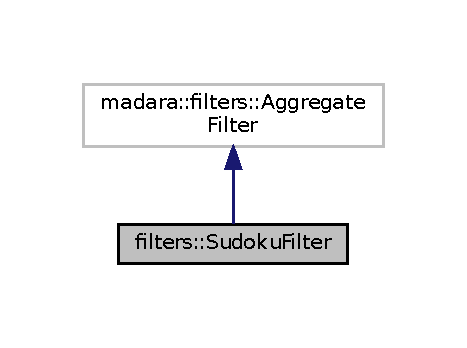
\includegraphics[width=224pt]{d5/d7f/classfilters_1_1SudokuFilter__inherit__graph}
\end{center}
\end{figure}


Collaboration diagram for filters\+:\+:Sudoku\+Filter\+:\nopagebreak
\begin{figure}[H]
\begin{center}
\leavevmode
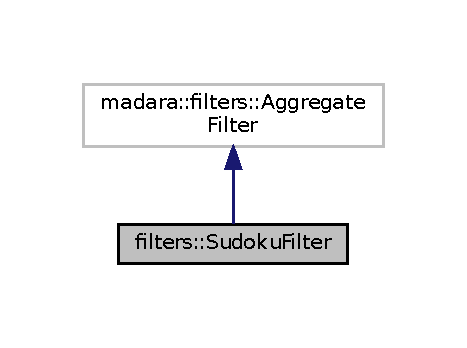
\includegraphics[width=224pt]{d5/d58/classfilters_1_1SudokuFilter__coll__graph}
\end{center}
\end{figure}
\subsection*{Public Member Functions}
\begin{DoxyCompactItemize}
\item 
\hyperlink{classfilters_1_1SudokuFilter_a2715aa3b65666655525028dd16ac2f8b}{Sudoku\+Filter} ()
\begin{DoxyCompactList}\small\item\em Constructor. \end{DoxyCompactList}\item 
virtual \hyperlink{classfilters_1_1SudokuFilter_afd43981e802eb6cceb68cdeb381a6d69}{$\sim$\+Sudoku\+Filter} ()
\begin{DoxyCompactList}\small\item\em Destructor. \end{DoxyCompactList}\item 
virtual void \hyperlink{classfilters_1_1SudokuFilter_a45e7f165bbed159d73c5784d1a53bf2a}{filter} (madara\+::knowledge\+::\+Knowledge\+Map \&records, const madara\+::transport\+::\+Transport\+Context \&transport\+\_\+context, madara\+::knowledge\+::\+Variables \&vars)
\begin{DoxyCompactList}\small\item\em The method that filters incoming or outgoing. \end{DoxyCompactList}\end{DoxyCompactItemize}


\subsection{Detailed Description}
A stateful filter generated by gpc.\+pl. 

Definition at line 14 of file Sudoku\+Filter.\+h.



\subsection{Constructor \& Destructor Documentation}
\mbox{\Hypertarget{classfilters_1_1SudokuFilter_a2715aa3b65666655525028dd16ac2f8b}\label{classfilters_1_1SudokuFilter_a2715aa3b65666655525028dd16ac2f8b}} 
\index{filters\+::\+Sudoku\+Filter@{filters\+::\+Sudoku\+Filter}!Sudoku\+Filter@{Sudoku\+Filter}}
\index{Sudoku\+Filter@{Sudoku\+Filter}!filters\+::\+Sudoku\+Filter@{filters\+::\+Sudoku\+Filter}}
\subsubsection{\texorpdfstring{Sudoku\+Filter()}{SudokuFilter()}}
{\footnotesize\ttfamily filters\+::\+Sudoku\+Filter\+::\+Sudoku\+Filter (\begin{DoxyParamCaption}{ }\end{DoxyParamCaption})}



Constructor. 



Definition at line 4 of file Sudoku\+Filter.\+cpp.

\mbox{\Hypertarget{classfilters_1_1SudokuFilter_afd43981e802eb6cceb68cdeb381a6d69}\label{classfilters_1_1SudokuFilter_afd43981e802eb6cceb68cdeb381a6d69}} 
\index{filters\+::\+Sudoku\+Filter@{filters\+::\+Sudoku\+Filter}!````~Sudoku\+Filter@{$\sim$\+Sudoku\+Filter}}
\index{````~Sudoku\+Filter@{$\sim$\+Sudoku\+Filter}!filters\+::\+Sudoku\+Filter@{filters\+::\+Sudoku\+Filter}}
\subsubsection{\texorpdfstring{$\sim$\+Sudoku\+Filter()}{~SudokuFilter()}}
{\footnotesize\ttfamily filters\+::\+Sudoku\+Filter\+::$\sim$\+Sudoku\+Filter (\begin{DoxyParamCaption}{ }\end{DoxyParamCaption})\hspace{0.3cm}{\ttfamily [virtual]}}



Destructor. 



Definition at line 8 of file Sudoku\+Filter.\+cpp.



\subsection{Member Function Documentation}
\mbox{\Hypertarget{classfilters_1_1SudokuFilter_a45e7f165bbed159d73c5784d1a53bf2a}\label{classfilters_1_1SudokuFilter_a45e7f165bbed159d73c5784d1a53bf2a}} 
\index{filters\+::\+Sudoku\+Filter@{filters\+::\+Sudoku\+Filter}!filter@{filter}}
\index{filter@{filter}!filters\+::\+Sudoku\+Filter@{filters\+::\+Sudoku\+Filter}}
\subsubsection{\texorpdfstring{filter()}{filter()}}
{\footnotesize\ttfamily void filters\+::\+Sudoku\+Filter\+::filter (\begin{DoxyParamCaption}\item[{madara\+::knowledge\+::\+Knowledge\+Map \&}]{records,  }\item[{const madara\+::transport\+::\+Transport\+Context \&}]{transport\+\_\+context,  }\item[{madara\+::knowledge\+::\+Variables \&}]{vars }\end{DoxyParamCaption})\hspace{0.3cm}{\ttfamily [virtual]}}



The method that filters incoming or outgoing. 


\begin{DoxyParams}{Parameters}
{\em records} & the aggregated packet being evaluated \\
\hline
{\em transport\+\_\+context} & context for querying transport state \\
\hline
{\em vars} & context for querying current program state \\
\hline
\end{DoxyParams}


Definition at line 13 of file Sudoku\+Filter.\+cpp.



The documentation for this class was generated from the following files\+:\begin{DoxyCompactItemize}
\item 
src/filters/\hyperlink{SudokuFilter_8h}{Sudoku\+Filter.\+h}\item 
src/filters/\hyperlink{SudokuFilter_8cpp}{Sudoku\+Filter.\+cpp}\end{DoxyCompactItemize}

\chapter{File Documentation}
\hypertarget{MainPage_8md}{}\section{docs/\+Main\+Page.md File Reference}
\label{MainPage_8md}\index{docs/\+Main\+Page.\+md@{docs/\+Main\+Page.\+md}}

\hypertarget{SudokuFilter_8cpp}{}\section{src/filters/\+Sudoku\+Filter.cpp File Reference}
\label{SudokuFilter_8cpp}\index{src/filters/\+Sudoku\+Filter.\+cpp@{src/filters/\+Sudoku\+Filter.\+cpp}}
{\ttfamily \#include \char`\"{}Sudoku\+Filter.\+h\char`\"{}}\newline
Include dependency graph for Sudoku\+Filter.\+cpp\+:\nopagebreak
\begin{figure}[H]
\begin{center}
\leavevmode
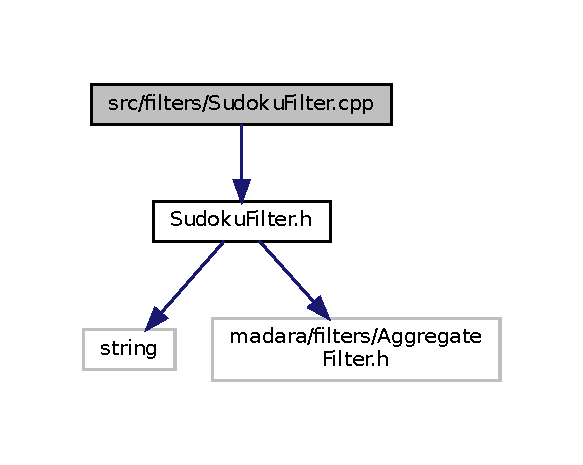
\includegraphics[width=280pt]{db/d28/SudokuFilter_8cpp__incl}
\end{center}
\end{figure}

\hypertarget{SudokuFilter_8h}{}\section{src/filters/\+Sudoku\+Filter.h File Reference}
\label{SudokuFilter_8h}\index{src/filters/\+Sudoku\+Filter.\+h@{src/filters/\+Sudoku\+Filter.\+h}}
{\ttfamily \#include $<$string$>$}\newline
{\ttfamily \#include \char`\"{}madara/filters/\+Aggregate\+Filter.\+h\char`\"{}}\newline
Include dependency graph for Sudoku\+Filter.\+h\+:\nopagebreak
\begin{figure}[H]
\begin{center}
\leavevmode
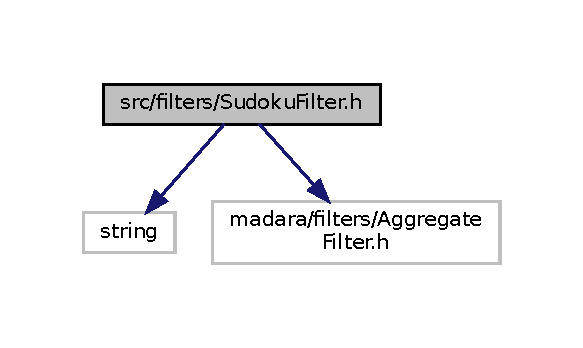
\includegraphics[width=280pt]{de/d18/SudokuFilter_8h__incl}
\end{center}
\end{figure}
This graph shows which files directly or indirectly include this file\+:\nopagebreak
\begin{figure}[H]
\begin{center}
\leavevmode
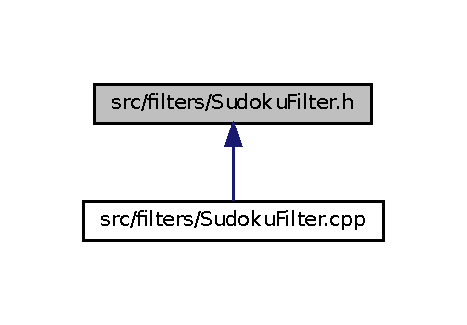
\includegraphics[width=224pt]{db/d8e/SudokuFilter_8h__dep__incl}
\end{center}
\end{figure}
\subsection*{Classes}
\begin{DoxyCompactItemize}
\item 
class \hyperlink{classfilters_1_1SudokuFilter}{filters\+::\+Sudoku\+Filter}
\begin{DoxyCompactList}\small\item\em A stateful filter generated by gpc.\+pl. \end{DoxyCompactList}\end{DoxyCompactItemize}
\subsection*{Namespaces}
\begin{DoxyCompactItemize}
\item 
 \hyperlink{namespacefilters}{filters}
\end{DoxyCompactItemize}

\hypertarget{sudoku__agent_8cpp}{}\section{src/sudoku\+\_\+agent.cpp File Reference}
\label{sudoku__agent_8cpp}\index{src/sudoku\+\_\+agent.\+cpp@{src/sudoku\+\_\+agent.\+cpp}}
{\ttfamily \#include $<$algorithm$>$}\newline
{\ttfamily \#include $<$future$>$}\newline
{\ttfamily \#include $<$iostream$>$}\newline
{\ttfamily \#include $<$sstream$>$}\newline
{\ttfamily \#include $<$string$>$}\newline
{\ttfamily \#include $<$unistd.\+h$>$}\newline
{\ttfamily \#include \char`\"{}madara/knowledge/\+Knowledge\+Base.\+h\char`\"{}}\newline
{\ttfamily \#include \char`\"{}madara/knowledge/containers/\+Flex\+Map.\+h\char`\"{}}\newline
{\ttfamily \#include \char`\"{}madara/knowledge/containers/\+Integer.\+h\char`\"{}}\newline
{\ttfamily \#include \char`\"{}madara/utility/\+Utility.\+h\char`\"{}}\newline
Include dependency graph for sudoku\+\_\+agent.\+cpp\+:\nopagebreak
\begin{figure}[H]
\begin{center}
\leavevmode
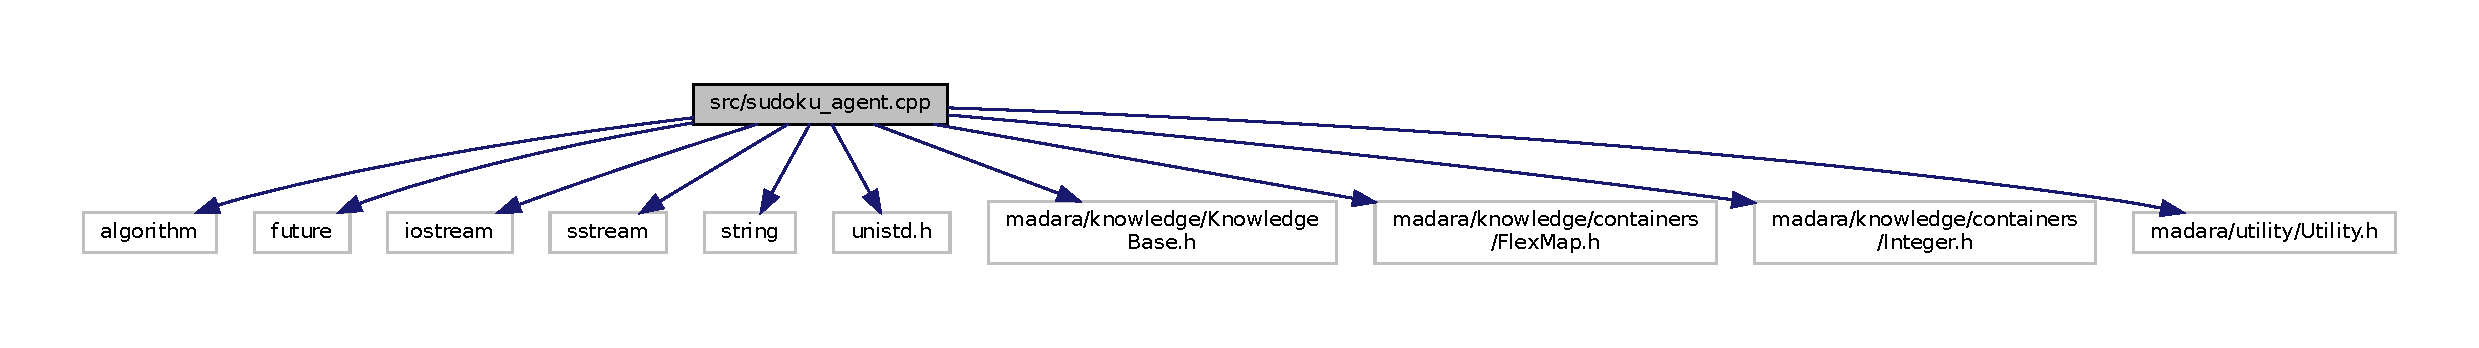
\includegraphics[width=350pt]{d9/df9/sudoku__agent_8cpp__incl}
\end{center}
\end{figure}
\subsection*{Typedefs}
\begin{DoxyCompactItemize}
\item 
typedef engine\+::\+Eval\+Settings \hyperlink{sudoku__agent_8cpp_aa3852b935f4e83fae32164c1922670a3}{Eval\+Settings}
\item 
typedef madara\+::transport\+::\+Qo\+S\+Transport\+Settings \hyperlink{sudoku__agent_8cpp_a94ded35bdf9aa42c18b166fbf2aa816d}{Qo\+S\+Transport\+Settings}
\end{DoxyCompactItemize}
\subsection*{Functions}
\begin{DoxyCompactItemize}
\item 
void \hyperlink{sudoku__agent_8cpp_a677f8ea0d1cd1a7aa388de5b18763a56}{add\+\_\+agent} (int id, \hyperlink{sudoku__agent_8cpp_a94ded35bdf9aa42c18b166fbf2aa816d}{Qo\+S\+Transport\+Settings} \&settings)
\begin{DoxyCompactList}\small\item\em Construct \mbox{[}protocol\mbox{]}\+://\mbox{[}ip\mbox{]}\+:\mbox{[}port\mbox{]} and push to settings.\+hosts. \end{DoxyCompactList}\item 
void \hyperlink{sudoku__agent_8cpp_a4a6f7757cbc7055fdd90cb67c5e64f01}{add\+\_\+peers} (int id, \hyperlink{sudoku__agent_8cpp_a94ded35bdf9aa42c18b166fbf2aa816d}{Qo\+S\+Transport\+Settings} \&settings)
\begin{DoxyCompactList}\small\item\em Add peers to settings.\+hosts (skipping this agent) \end{DoxyCompactList}\item 
int \hyperlink{sudoku__agent_8cpp_ab1fa5b2074bb27f45e5fc02e5bcba6bc}{find\+\_\+value} (containers\+::\+Integer id, containers\+::\+Flex\+Map \&agents)
\begin{DoxyCompactList}\small\item\em Check peers in same row/col/quad to find value by process of elimination. \end{DoxyCompactList}\item 
std\+::string \hyperlink{sudoku__agent_8cpp_a982f4a462e23a5b6d37f88f16de65200}{host} (\char`\"{}\char`\"{})
\item 
std\+::string \hyperlink{sudoku__agent_8cpp_af9fd3267763c52bb7d35d20600d68b81}{host\+\_\+prefix} (\char`\"{}tcp\+://127.\+0.\+0.\+1\+:\char`\"{})
\item 
bool \hyperlink{sudoku__agent_8cpp_aeaaeb32f3bcdfcd91a58c6151d87a769}{is\+\_\+complete} (containers\+::\+Flex\+Map \&agents)
\begin{DoxyCompactList}\small\item\em Check that all agents have a non-\/zero value. \end{DoxyCompactList}\item 
int \hyperlink{sudoku__agent_8cpp_a0ddf1224851353fc92bfbff6f499fa97}{main} (int argc, char $\ast$argv\mbox{[}$\,$\mbox{]})
\begin{DoxyCompactList}\small\item\em Entry point to sudoku agent. \end{DoxyCompactList}\end{DoxyCompactItemize}
\subsection*{Variables}
\begin{DoxyCompactItemize}
\item 
int \hyperlink{sudoku__agent_8cpp_a986befd442815886b539653b02cca566}{num\+\_\+agents} = 81
\item 
int \hyperlink{sudoku__agent_8cpp_a43f552b00d972f4ef1538bf089007ba9}{starting\+\_\+port} = 30000
\end{DoxyCompactItemize}


\subsection{Detailed Description}
\begin{DoxyAuthor}{Author}
Eric Adlam \href{mailto:eadlam@gmail.com}{\tt eadlam@gmail.\+com}
\end{DoxyAuthor}
This is the entry point and contains all functions and definitions for Madara Sudoku 

\subsection{Typedef Documentation}
\mbox{\Hypertarget{sudoku__agent_8cpp_aa3852b935f4e83fae32164c1922670a3}\label{sudoku__agent_8cpp_aa3852b935f4e83fae32164c1922670a3}} 
\index{sudoku\+\_\+agent.\+cpp@{sudoku\+\_\+agent.\+cpp}!Eval\+Settings@{Eval\+Settings}}
\index{Eval\+Settings@{Eval\+Settings}!sudoku\+\_\+agent.\+cpp@{sudoku\+\_\+agent.\+cpp}}
\subsubsection{\texorpdfstring{Eval\+Settings}{EvalSettings}}
{\footnotesize\ttfamily typedef engine\+::\+Eval\+Settings \hyperlink{sudoku__agent_8cpp_aa3852b935f4e83fae32164c1922670a3}{Eval\+Settings}}



Definition at line 24 of file sudoku\+\_\+agent.\+cpp.

\mbox{\Hypertarget{sudoku__agent_8cpp_a94ded35bdf9aa42c18b166fbf2aa816d}\label{sudoku__agent_8cpp_a94ded35bdf9aa42c18b166fbf2aa816d}} 
\index{sudoku\+\_\+agent.\+cpp@{sudoku\+\_\+agent.\+cpp}!Qo\+S\+Transport\+Settings@{Qo\+S\+Transport\+Settings}}
\index{Qo\+S\+Transport\+Settings@{Qo\+S\+Transport\+Settings}!sudoku\+\_\+agent.\+cpp@{sudoku\+\_\+agent.\+cpp}}
\subsubsection{\texorpdfstring{Qo\+S\+Transport\+Settings}{QoSTransportSettings}}
{\footnotesize\ttfamily typedef madara\+::transport\+::\+Qo\+S\+Transport\+Settings \hyperlink{sudoku__agent_8cpp_a94ded35bdf9aa42c18b166fbf2aa816d}{Qo\+S\+Transport\+Settings}}



Definition at line 25 of file sudoku\+\_\+agent.\+cpp.



\subsection{Function Documentation}
\mbox{\Hypertarget{sudoku__agent_8cpp_a677f8ea0d1cd1a7aa388de5b18763a56}\label{sudoku__agent_8cpp_a677f8ea0d1cd1a7aa388de5b18763a56}} 
\index{sudoku\+\_\+agent.\+cpp@{sudoku\+\_\+agent.\+cpp}!add\+\_\+agent@{add\+\_\+agent}}
\index{add\+\_\+agent@{add\+\_\+agent}!sudoku\+\_\+agent.\+cpp@{sudoku\+\_\+agent.\+cpp}}
\subsubsection{\texorpdfstring{add\+\_\+agent()}{add\_agent()}}
{\footnotesize\ttfamily void add\+\_\+agent (\begin{DoxyParamCaption}\item[{int}]{id,  }\item[{\hyperlink{sudoku__agent_8cpp_a94ded35bdf9aa42c18b166fbf2aa816d}{Qo\+S\+Transport\+Settings} \&}]{settings }\end{DoxyParamCaption})}



Construct \mbox{[}protocol\mbox{]}\+://\mbox{[}ip\mbox{]}\+:\mbox{[}port\mbox{]} and push to settings.\+hosts. 


\begin{DoxyParams}[1]{Parameters}
\mbox{\tt in}  & {\em id} & Add id to starting port to get port number \\
\hline
\mbox{\tt out}  & {\em settings} & The address is pushed to settings.\+hosts \\
\hline
\end{DoxyParams}


Definition at line 49 of file sudoku\+\_\+agent.\+cpp.

\mbox{\Hypertarget{sudoku__agent_8cpp_a4a6f7757cbc7055fdd90cb67c5e64f01}\label{sudoku__agent_8cpp_a4a6f7757cbc7055fdd90cb67c5e64f01}} 
\index{sudoku\+\_\+agent.\+cpp@{sudoku\+\_\+agent.\+cpp}!add\+\_\+peers@{add\+\_\+peers}}
\index{add\+\_\+peers@{add\+\_\+peers}!sudoku\+\_\+agent.\+cpp@{sudoku\+\_\+agent.\+cpp}}
\subsubsection{\texorpdfstring{add\+\_\+peers()}{add\_peers()}}
{\footnotesize\ttfamily void add\+\_\+peers (\begin{DoxyParamCaption}\item[{int}]{id,  }\item[{\hyperlink{sudoku__agent_8cpp_a94ded35bdf9aa42c18b166fbf2aa816d}{Qo\+S\+Transport\+Settings} \&}]{settings }\end{DoxyParamCaption})}



Add peers to settings.\+hosts (skipping this agent) 

The transport layer expects the current agent to be the first item in settings.\+hosts, and for peers to follow. This adds all peers, skipping the current agent


\begin{DoxyParams}[1]{Parameters}
\mbox{\tt in}  & {\em id} & The id of the current agent to skip \\
\hline
\mbox{\tt out}  & {\em settings} & The peers are pushed to settings.\+hosts \\
\hline
\end{DoxyParams}


Definition at line 65 of file sudoku\+\_\+agent.\+cpp.

\mbox{\Hypertarget{sudoku__agent_8cpp_ab1fa5b2074bb27f45e5fc02e5bcba6bc}\label{sudoku__agent_8cpp_ab1fa5b2074bb27f45e5fc02e5bcba6bc}} 
\index{sudoku\+\_\+agent.\+cpp@{sudoku\+\_\+agent.\+cpp}!find\+\_\+value@{find\+\_\+value}}
\index{find\+\_\+value@{find\+\_\+value}!sudoku\+\_\+agent.\+cpp@{sudoku\+\_\+agent.\+cpp}}
\subsubsection{\texorpdfstring{find\+\_\+value()}{find\_value()}}
{\footnotesize\ttfamily int find\+\_\+value (\begin{DoxyParamCaption}\item[{containers\+::\+Integer}]{id,  }\item[{containers\+::\+Flex\+Map \&}]{agents }\end{DoxyParamCaption})}



Check peers in same row/col/quad to find value by process of elimination. 


\begin{DoxyParams}[1]{Parameters}
\mbox{\tt in}  & {\em id} & The id of the current agent \\
\hline
\mbox{\tt in,out}  & {\em agents} & The object to search and update \\
\hline
\end{DoxyParams}
Search over all agents, ignoring those that are not in same row/col/quad

Check if all but one were eliminated

values are 1-\/9, so add 1 to the index 

Definition at line 81 of file sudoku\+\_\+agent.\+cpp.

\mbox{\Hypertarget{sudoku__agent_8cpp_a982f4a462e23a5b6d37f88f16de65200}\label{sudoku__agent_8cpp_a982f4a462e23a5b6d37f88f16de65200}} 
\index{sudoku\+\_\+agent.\+cpp@{sudoku\+\_\+agent.\+cpp}!host@{host}}
\index{host@{host}!sudoku\+\_\+agent.\+cpp@{sudoku\+\_\+agent.\+cpp}}
\subsubsection{\texorpdfstring{host()}{host()}}
{\footnotesize\ttfamily std\+::string host (\begin{DoxyParamCaption}\item[{\char`\"{}\char`\"{}}]{ }\end{DoxyParamCaption})}

\mbox{\Hypertarget{sudoku__agent_8cpp_af9fd3267763c52bb7d35d20600d68b81}\label{sudoku__agent_8cpp_af9fd3267763c52bb7d35d20600d68b81}} 
\index{sudoku\+\_\+agent.\+cpp@{sudoku\+\_\+agent.\+cpp}!host\+\_\+prefix@{host\+\_\+prefix}}
\index{host\+\_\+prefix@{host\+\_\+prefix}!sudoku\+\_\+agent.\+cpp@{sudoku\+\_\+agent.\+cpp}}
\subsubsection{\texorpdfstring{host\+\_\+prefix()}{host\_prefix()}}
{\footnotesize\ttfamily std\+::string host\+\_\+prefix (\begin{DoxyParamCaption}\item[{\char`\"{}tcp\+://127.\+0.\+0.\+1\+:\char`\"{}}]{ }\end{DoxyParamCaption})}

\mbox{\Hypertarget{sudoku__agent_8cpp_aeaaeb32f3bcdfcd91a58c6151d87a769}\label{sudoku__agent_8cpp_aeaaeb32f3bcdfcd91a58c6151d87a769}} 
\index{sudoku\+\_\+agent.\+cpp@{sudoku\+\_\+agent.\+cpp}!is\+\_\+complete@{is\+\_\+complete}}
\index{is\+\_\+complete@{is\+\_\+complete}!sudoku\+\_\+agent.\+cpp@{sudoku\+\_\+agent.\+cpp}}
\subsubsection{\texorpdfstring{is\+\_\+complete()}{is\_complete()}}
{\footnotesize\ttfamily bool is\+\_\+complete (\begin{DoxyParamCaption}\item[{containers\+::\+Flex\+Map \&}]{agents }\end{DoxyParamCaption})}



Check that all agents have a non-\/zero value. 


\begin{DoxyParams}[1]{Parameters}
\mbox{\tt in,out}  & {\em agents} & The object to search and update \\
\hline
\end{DoxyParams}


Definition at line 117 of file sudoku\+\_\+agent.\+cpp.

\mbox{\Hypertarget{sudoku__agent_8cpp_a0ddf1224851353fc92bfbff6f499fa97}\label{sudoku__agent_8cpp_a0ddf1224851353fc92bfbff6f499fa97}} 
\index{sudoku\+\_\+agent.\+cpp@{sudoku\+\_\+agent.\+cpp}!main@{main}}
\index{main@{main}!sudoku\+\_\+agent.\+cpp@{sudoku\+\_\+agent.\+cpp}}
\subsubsection{\texorpdfstring{main()}{main()}}
{\footnotesize\ttfamily int main (\begin{DoxyParamCaption}\item[{int}]{argc,  }\item[{char $\ast$}]{argv\mbox{[}$\,$\mbox{]} }\end{DoxyParamCaption})}



Entry point to sudoku agent. 

For simplicity, I\textquotesingle{}m just assuming both arguments are passed as expected

Setup Z\+MQ network

Initialize knowledgebase and agent id

setup private knowledge variables / calculate row, col, quadrant

setup global knowledge variables

until complete, keep propogating/deducing info

Propogate row, col, quad, value

If our value is 0, check peers and try to update value

If solution is complete, set complete flag and save to file 

Definition at line 135 of file sudoku\+\_\+agent.\+cpp.



\subsection{Variable Documentation}
\mbox{\Hypertarget{sudoku__agent_8cpp_a986befd442815886b539653b02cca566}\label{sudoku__agent_8cpp_a986befd442815886b539653b02cca566}} 
\index{sudoku\+\_\+agent.\+cpp@{sudoku\+\_\+agent.\+cpp}!num\+\_\+agents@{num\+\_\+agents}}
\index{num\+\_\+agents@{num\+\_\+agents}!sudoku\+\_\+agent.\+cpp@{sudoku\+\_\+agent.\+cpp}}
\subsubsection{\texorpdfstring{num\+\_\+agents}{num\_agents}}
{\footnotesize\ttfamily int num\+\_\+agents = 81}



Definition at line 32 of file sudoku\+\_\+agent.\+cpp.

\mbox{\Hypertarget{sudoku__agent_8cpp_a43f552b00d972f4ef1538bf089007ba9}\label{sudoku__agent_8cpp_a43f552b00d972f4ef1538bf089007ba9}} 
\index{sudoku\+\_\+agent.\+cpp@{sudoku\+\_\+agent.\+cpp}!starting\+\_\+port@{starting\+\_\+port}}
\index{starting\+\_\+port@{starting\+\_\+port}!sudoku\+\_\+agent.\+cpp@{sudoku\+\_\+agent.\+cpp}}
\subsubsection{\texorpdfstring{starting\+\_\+port}{starting\_port}}
{\footnotesize\ttfamily int starting\+\_\+port = 30000}



Definition at line 31 of file sudoku\+\_\+agent.\+cpp.


%--- End generated contents ---

% Index
\backmatter
\newpage
\phantomsection
\clearemptydoublepage
\addcontentsline{toc}{chapter}{Index}
\printindex

\end{document}
